\section{Introduction}
Bitcoin and other currencies often debate the inclusion of new features in the
consensus layer. Such upgrades can be implemented via soft-, hard-, or
velvet-forks. In the case of a soft- or hard-fork, it is typical to ask for
the opinion of the miners before an upgrade can be activated (unless the
fork is user-activated, in which case a miner census is not taken). This
process, known as \emph{activation signaling}, is implemented using the
following process:

\begin{enumerate}
  \item Initially, the proposal is posted on an \emph{off-chain} public forum
        such as GitHub. The proposal specifies the desired protocol upgrade, the
        type of fork proposed, and its parameters. The parameters include the
        \emph{signaling period}, which has a designated \emph{beginning block
        height} $j_0$ and \emph{ending block height} $j_1$. A designated
        \emph{lock-in block height} $j_2$ is also provided, with
        $j_2 > j_1 + k$.
  \item During the signaling period, each miner is able to vote \emph{for}  the
        proposal by flipping a flag in their coinbase transaction in every block
        they generate in their reported portion of the chain $\chain[j_0:j_1]$.
        Votes in blocks outside the signaling period are ignored. Abstaining
        from a vote is counted as a vote \emph{against} the proposal. The
        rationale is that the miner is either unaware or unwilling to go forward
        with the proposal, hence adoption will be hindered.
  \item Once the signaling period has been designated as \emph{stable} by being
        buried under $k$ blocks, the votes are counted.
  \item If the votes in the signaling period exceed a certain
        \emph{supermajority} $\phi$, the voting is considered successful and the
        proposal is passed, starting with block $\chain[j_2]$. Each honest miner
        who has voted \emph{for} the protocol therefore counts the number of
        blocks with the flag flipped in their adopted chain $\chain[j_0:j_1]$
        and activates the code running the new protocol if the threshold is
        surpassed.
\end{enumerate}

Miners who are aware of the protocol but have abstained from voting are
encouraged to respect the majority who have voted in favour and adopt the new
code. Miners who are unaware of the proposal or who do not wish to upgrade
despite the majority vote are forced to upgrade as follows. If the upgrade is a
hard-fork, the minority miners will keep extending an outdated chain, causing
a chain split; in practice, the economic majority will typically move to the
upgraded chain and the mining rewards of the minority will be worth
little~\footnote{One exception to this are cases where coins have survived a
hard fork split and new coins were created; an example is Ethereum and Ethereum
Classic}. In the case of a soft-fork, the outdated miners will generate blocks
which the supermajority will not accept. Hence, they will be completely deprived
of their payments. It has been argued that this economic mechanism incentivizes
the minority to go along with the majority~\cite{vitalik-forks}.

In bitcoin, the supermajority is typically defined to require
$\phi = 95\%$~\cite{BIP9}, but often \emph{reduced threshold values} as low as
$\phi = 80\%$~\cite{BIP141} have been put forth for proposals which the
developers wanted to push forward. Beginning and ending block heights can either
be given as block heights or as UNIX timestamps. Typical values for Bitcoin's
$j_2 - j_1$ range from $24048$~\cite{BIP91} to $52560$~\cite{BIP141}.

Consider the predicate $p(B)$ indicating that block $B$ contains a flipped flag
voting \emph{for} the proposed change. Suppose that the required supermajority
threshold is $\phi$. The voting outcome according to the view of an honest party
with adopted chain $\chain$ with $|\chain| > j_1$ is therefore
$|\{B \in \chain[j_0:j_1]: p(B)\}| \geq \phi(j_2 - j_1)$. We observe that $p$ is
a moustache predicate.

Consider an adversary controlling $t / n$ mining power, and suppose this
adversary is \emph{in favour} of the upcoming proposal (the case where the
adversary is \emph{against} is symmetric). The adversary tries to suppress the
voice of the minority in order to cause a supermajority to appear to be winning,
even though the actual opinion of the population may be different. The questions
we will try to answer are:

\begin{enumerate}
  \item What is the required \emph{actual opinion} $\max\theta < \phi$
        needed among all parties such that this adversary is able to swing the
        election so that at least a $\phi$ percentage appears to be in favour of
        the proposal?
  \item Given a particular $\phi$, can we certainly deduce that a particular
        $\min\theta < \phi$ of the population agrees with the apparent opinion?
\end{enumerate}

For a reference to these quantities, see
Figure~\ref{figure:signalling-percentages}. The adversary, whose computational
power percantage is shown in black, wishes to sway the public vote in favour of
a protocol proposal. The honest parties are divided regarding the vote; some of
them (gray) are in favour of the proposal, while others (white) are against. The
total \emph{actual} computational power against the proposal, including the
adversary, is marked by $\theta$. It is therefore impossible for the adversary
to cause the apparant public opinion to reach $\phi$, the required
supermajority. If the actual public opinion was at least $\max\theta$, the
adversary could cause the apparent opinion to reach $\phi$. If an honest party
observes an apparent opinion of at least $\phi$ in favour of the opinion,
they deduce that the actual percentage must be at least $\min\theta$.

This establishes two bounds for $\theta$: On the lower end, we know that no
adversary is able to achieve an apparent public opinion of $\phi$ unless
$\min\theta$ is achieved. This impossibility result is established from the
moustaches theorems. On the higher end, we know that no more than $\max\theta$
is required for an adversary to achieve $\phi$. This result is established by
measuring the probability of success in an actual attack through simulation. The
gap between $\min\theta$ and $\max\theta$ (shown in striped pattern) exists
because there could be better attacks for swaying the vote.

\begin{figure*}[h]
\begin{center}
    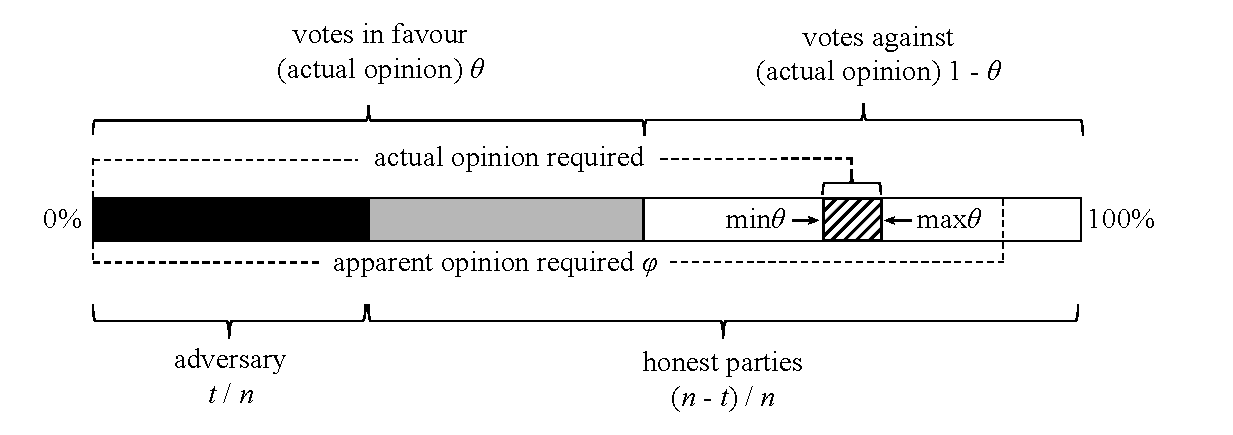
\includegraphics[width=0.95\textwidth]{figures/signalling-percentages.pdf}
  \caption{The various thresholds in a proof-of-work signaling scheme.}
  \label{fig:signalling-percentages}
  \end{center}
\end{figure*}

% TODO: what is our relationship with fruitchains here?
